\chapter{Preliminaries}\label{ch:preliminaries}

\section{Types of machine learning}
\label{sec:prelim:types-of-machine-learning}

There are different approaches to machine learning. In this section we will introduce a few of these approaches to give context for our research.


\subsection{Supervised learning}

Supervised learning \cite{mohri_foundations_2012} is a type of machine learning approach that always uses a labeled dataset to train a model. This means that for each point in the dataset we already know what class or rank it belongs to. It is the common type of learning used with problems that require classification, regression or ranking. The known samples are used to train a model and to make predictions for data points that the model has not yet seen.

An example would be making predictions about images of animals. Each image would be labeled with the type of animal that is in the picture. Use that data we would be learning our models to be able to predict the type of animal in pictures that the model has never seen before.

\subsection{Unsupervised learning}

This subset of machine learning focuses on training models with unlabeled data. Examples of problems that use this type of learning are clustering and dimensionality reduction. For unsupervised methods it is hard to measure the performance quantitatively because there are no labels to compare the results to.

An example of this type would be clustering people by known information like age, education or income. The goal here is to split the dataset based on information that is similar between the points. So only the points from the dataset are used to create a result, there is no previous knowledge about the data that can be used.

\subsection{Self-supervised learning}

The type of machine learning that we use in this thesis is a form of self-supervised learning \cite{doersch_multi-task_2017}. This means that we generate our own labels from a dataset without any manual work required. This is possible by removing or modifying part of the input data and then learn a model to recover the original data. We can measure the performance based on the difference between the original data and the result. This type of learning can be seen as a combination of unsupervised and supervised learning.

An example is a model that tries to predict words in a certain context. We have a sentence: 'The most popular food from France is the croissant'. We can then leave out the word 'croissant' and train a model to predict the word based on the words surrounding it.

\section{Transformers}
\label{sec:prelim:transformers}

The type of model used in our research is a transformer. In this section we will introduce the attention mechanism, explain how this is used in transformers and how this is affecting the kind of transformer we are using.

\subsection{Vanilla transformers}
\label{sec:prelim:transformers:vanilla}

In 2017 Vaswani et al.\cite{vaswani_attention_2017} introduced the transformer model. A type of sequence to sequence model that uses an attention mechanism as the main building block. This allowed them to increase parallelisation and reach a new state of the art in the context of language translations.

\subsubsection{Architecture}

The transformer model uses the same encoder-decoder structure used in the models it was compared to in the original paper \cite{bahdanau_neural_2016, cho_learning_2014}. This means that the model consists of two parts: an encoder and a decoder.

The encoder takes an input representation $(x_1,...x_n)$ and transforms this to an intermediary representation $(z_1,...z_n)$. This intermediary representation is then used as input for the decoder to create an output $(y_1,...,y_n)$.

\begin{figure}[ht]
\centering
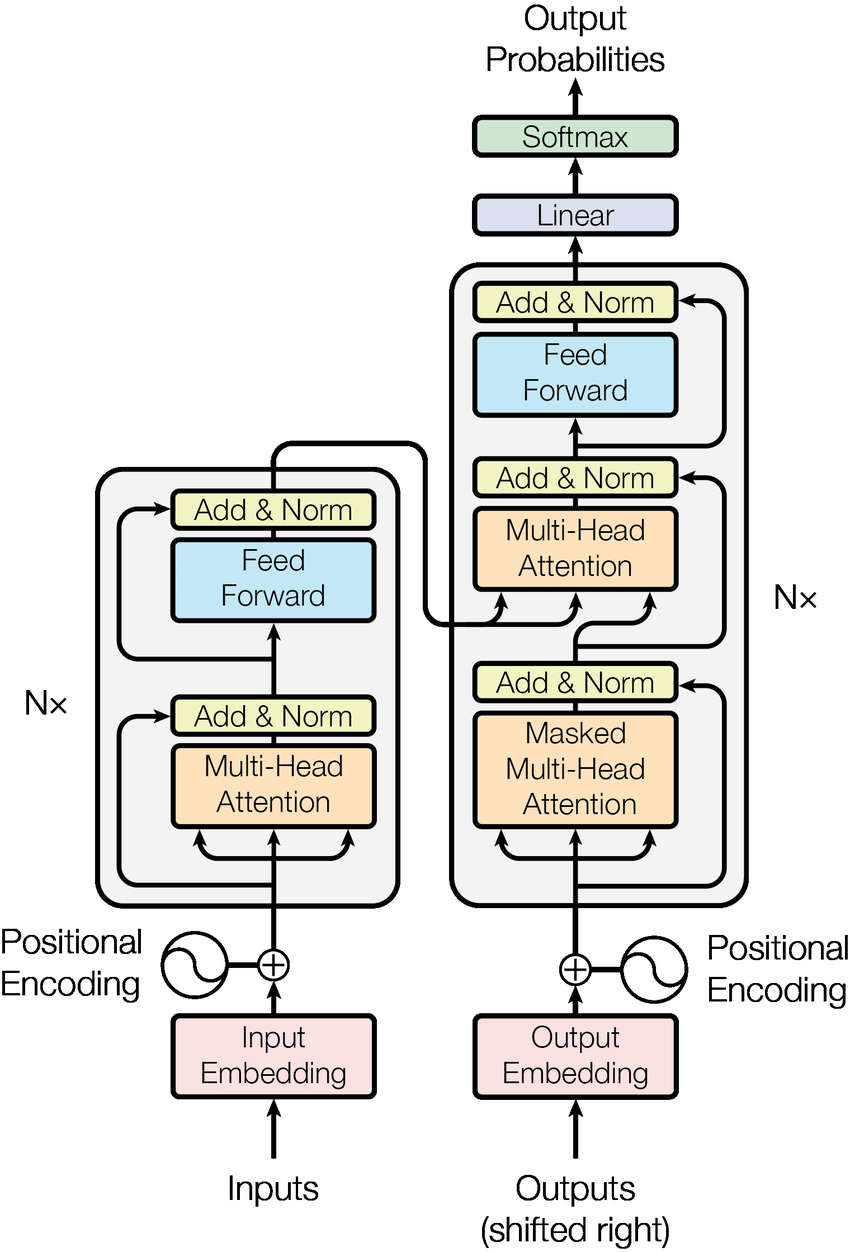
\includegraphics[width=0.5\textwidth]{transformer.png}
\caption{The original transformer architecture from \cite{vaswani_attention_2017}}
\label{fig:prelim:transformer-architecture}
\end{figure}


\paragraph{Attention}

The attention mechanism, which takes query, keys and values vector as input, outputs a vector containing a weighted sum of the values. Each of the output values uses a weight that is calculated using a compatibility  function of the query and the key in each position.

The attention mechanism \cite{vaswani_attention_2017} is called 'Scaled Dot-Product Attention' or softmax attention and calculates attention using matrices that consist of multiple vectors packed together. These matrices are $Q$ (queries), $K$ (keys) and $V$ (values) of dimension $S \times d_k$, $d_k \times S$ and $S \times d_v$ where $S$ is the sequence length of vectors:
\begin{align}
\label{eq:prelim:softmax-attention}
&Attention(Q, K, V) = softmax(\frac{QK^T} {\sqrt{d_k}})V
\end{align}

To be able to apply the attention to more than one representation space we use multi-headed attention. This uses $h$ parallel layers that all attend to a smaller part of the full dimension. In the case of the original papers $h = 8$ and the dimension of each attention head becomes $d_k = d_v = D / h = 64$ when $D = 512$. This makes the multi-headed attention similar to single-head attention with the full dimension when we look at the computational cost.

To combine the results of the attention heads we learn linear projections ($W_i^Q$, $W_i^K$, $W_i^V$) that we project all queries, keys and values to. All the separate outputs of the different attention heads are concatenated and projected into the correct dimension , which gives us the final output.

\begin{align}
&MultiHead(Q, K, V) = Concat(head_1, ..., head_h)W^O\\
& where\ head_i = Attention(QW_i^Q, KW_i^K, VW_i^V)
\end{align}


\paragraph{Encoder}
The encoder part in the architecture is a stack of $N$ layers. All the layers are the same and consist of two sublayers: the multi-head self-attention and a fully-connected feed-forward network (FFN). After both sublayers we apply layer normalisation\cite{ba_layer_2016} and add residual connections\cite{he_deep_2015} around the sublayers. This means that the output of a layer in the encoder is calculated as follows: 
\begin{align}
\label{par:prelim:transformer-encoder}
&selfAtt = LayerNorm(input + MultiHead(input_q, input_k, input_v))\\
&enc = LayerNorm(selfAtt + FFN(selfAtt))
\end{align}

where $input_q = input_k = input_v$ are the input of the encoder layer. These arguments are the same, since we are applying self-attention here.


\paragraph{Decoder}
Similar to the encoder the decoder is a stack of $N$ layers. Compared to the encoder it adds a third sublayer that applies multi-head cross attention to the output from the encoder layers and the first sublayer of the decoder. In the first self-attention sublayer we mask out earlier positions in the output sequence to stop predictions for a certain position $i$ to depend on the outputs at the positions before position $i$. The residual connections and layer normalisation on each sublayer is identical to the architecture of the encoder. This results in the following calculations for each decoder layer: 
\begin{align}
&selfAtt = LayerNorm(input + MaskedSelfAtt(input_q, input_k, input_v))\\
&crossAtt = LayerNorm(selfAtt + CrossAtt(selfAtt_q, enc_k, enc_v))\\
&dec = LayerNorm(crossAtt + FFN(crossAtt))
\end{align}

where $MaskedSelfAtt$ is the function that applies the masking before $MultiHead$, $input_q = input_k = input_v$ are the input of the decoder layer and $enc_k$ and $enc_v$ the keys and values of the encoder layers. $selfAtt_q$ are the queries from the first attention function.

The final layers consist of a linear fully connected neural network and a softmax layer. This allows us to have a higher number of possible outputs than the size of the input and output embeddings since it projects the output of the decoder part into a probability vector.

\subsection{Vision transformers}
\label{sec:prelim:transformers:vision}

As mentioned in the previous section transformers were originally meant for text problems. The success of the transformer in that context is what made Dosovitskiy et al. \cite{dosovitskiy_image_2021} start exploring the usage of the attention-based model for computer vision tasks as well.

Their approach tries to use the original transformer implementation as much as possible. This means that they had to introduce an intermediate step to be able to use the images as input for the model.

The original model is designed to receive a 1 dimensional input of token embeddings. The input images for the vision transformers are 2 dimensional and each image has the shape $x \in \mathbb{R}^{H \times W \times C}$ where $H$ and $W$ are the height and width of the image respectively and $C$ is the number of channels. To be able to use the images as input they split the image in square patches with the resolution $(P, P)$. This results in $N = HW/P^2$ patches $x_p \in \mathbb{R}^{N \times (P^2 \; \cdot \; C)}$.

To obtain the patch embeddings they first flatten the patches and then train a linear projection  mapping them to a single dimension. To this sequence of patch embeddings they prepend a learnable embedding. Then to allow for the preservation the positions of the patches, they add positional embeddings to the patch embeddings.

\subsection{Linear transformers}
\label{sec:prelim:transformers:linear}

Since transformers use attention to process so many parts of the images the model has a high memory and time complexity. One of the proposed solutions to reduce the complexity of the models is made by Katharopoulos et al. \cite{katharopoulos_transformers_2020}. They introduce the linear transformer that according to their results can reach similar performance when compared to vanilla transformers with the benefit of being faster. 

To see the advantage of their attention function we first need to understand what the bottleneck is in regular transformers. For this we look at equation \ref{eq:prelim:softmax-attention} again:

\begin{align}
&Attention(Q, K, V) = softmax(\frac{QK^T} {\sqrt{d_k}})V
\tag{\ref{eq:prelim:softmax-attention} revisited}
\end{align}

Here we apply the softmax function row-wise to $\frac{QK^T} {\sqrt{d_k}}$. This means that the complexity of the multiplication of the three matrices $Q$, $K^T$ and $V$ becomes $O(S^2 d_k)$.

The approach by Katharopoulus et al. starts by rewriting the attention calculation in equation \ref{eq:prelim:softmax-attention} into a generalised equation for any similarity function $sim(Q, K)$.

\begin{align}
&Attention(Q, K, V) = V'
\end{align}

Given that $V_i$ returns the i-th row of $V'$ as a vector:

\begin{align}
&V'_i =\frac{\sum_{j-1} ^{N} sim(Q_i, K_j) V_j}{\sum_{j-1} ^{N} sim(Q_i, K_j)}
\label{eq:prelim:general-attention}
\end{align}

This equation is equivalent to equation \ref{eq:prelim:softmax-attention} when we say $sim(q, k) = exp(\frac{q^Tk}{\sqrt{D}})$.

\\We need to set a constraint on $sim(q, k)$ for this equation to be able to define an attention function. And that is that it has to be non-negative.\\

Now given some kernel with a feature representation $\phi(x)$ we can rewrite equation \ref{eq:prelim:general-attention} as follows:

\begin{align}
    &V'_i = \frac{\sum_{j=1}^{N} \phi(Q_i)^T\phi(K_j)V_j}{\sum_{j=1}^{N} \phi(Q_i)^T\phi(K_j)}
    \label{eq:prelim:lin-att-1}
\end{align}

This is possible by using the kernel trick\footnote{https://en.wikipedia.org/wiki/Kernel_method#Mathematics:_the_kernel_trick}. We can avoid learning a non-linear function using this trick. It allows us to rewrite our similarity function as follows:

\begin{align}
sim(q, k) = \phi(q)^T\phi(k)
\end{align}

We can then simplify equation \ref{eq:prelim:lin-att-1} using the associative property of matrix multiplication to:

\begin{align}
    &V'_i = \frac{\phi(Q_i)^T\sum_{j=1}^{N} \phi(K_j)V_j^T}{\phi(Q_i)^T\sum_{j=1}^{N} \phi(K_j)}
\end{align}

In \cite{katharopoulos_transformers_2020} they note that the feature function $\phi(x)$ that corresponds to the exponential kernel $exp$ is infinite dimensional. This makes it infeasible to linearise softmax attention itself. Therefore they choose the following feature map:

\begin{align}
    \phi(x) = elu(x) + 1
\end{align}

with $elu(x)$ being the exponential linear unit activation function \cite{clevert_fast_2015}:

\begin{align}
    elu(x) =     \begin{cases}     \mbox{$x$} & \mbox{if } x > 0\\     \mbox{$\alpha (e^x-1)$} & \mbox{if } x < 0     \end{cases}
\end{align}

where $\alpha = 1.0$. This results in a complexity of $O(S d_k)$ which is no longer quadratic when compared to softmax attention.

\section{Image inpainting}
\label{sec:prelim:image-inpainting}

To be able to detect anomalies without labelling a large dataset we are using a semi-supervised method using image inpainting.

Inpainting is the process of filling in missing, damaged or censored parts in paintings or images. It can also be used for object removal or image manipulation.
Applying the technique on digital images can be done using different approaches.

\begin{figure}[ht!]
\centering
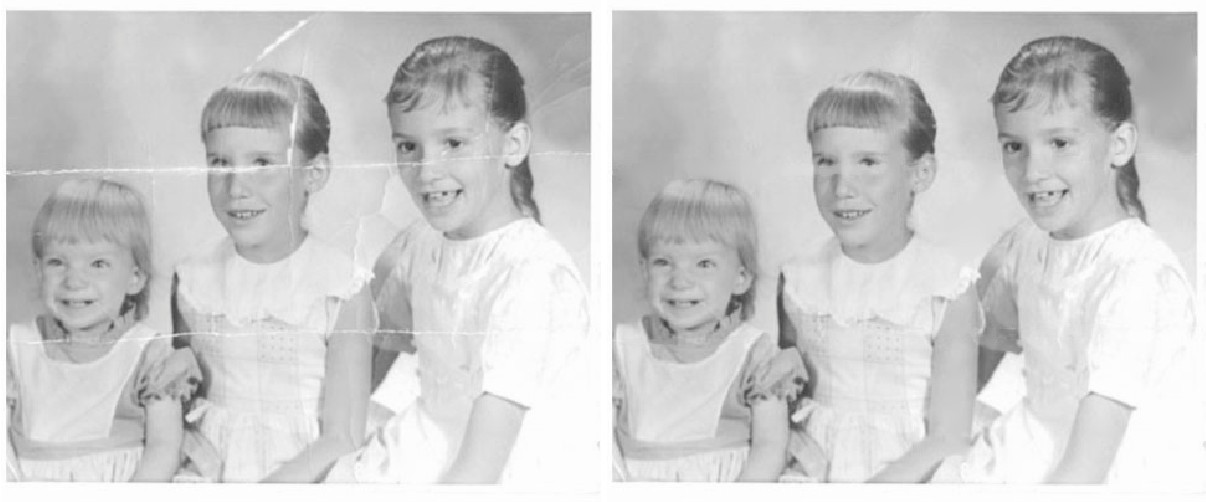
\includegraphics[width=\textwidth]{imgs/inpainting-example.jpeg}
\caption{An example of image restoration using inpainting from Bertalmio et al. \cite{bertalmio_image_2000}}
\label{fig:prelim:inpainting-example}
\end{figure}

In figure \ref{fig:prelim:inpainting-example} we see a photo that is restored by using a context based inpainting method.

Our transformer-based approach, which is modeled after the Inpainting Transformer (InTra) from Pirnay et al. \cite{pirnay_inpainting_2021} learns to paint regions that are removed from the original images. This allows the models to fully reconstruct an image based on the surrounding patches. This approach is discussed more extensively in section \ref{sec:experimental-setup:model}.

\section{Anomaly detection}
\label{sec:prelim:anomaly-detection}

Anomaly detection is the detection of outliers, points that have extreme values compared to the rest, in a dataset.
This kind of detection can be useful in different environments. Examples are intrusion detection in security and fault detection in industrial systems.

\begin{figure}[H]
\centering
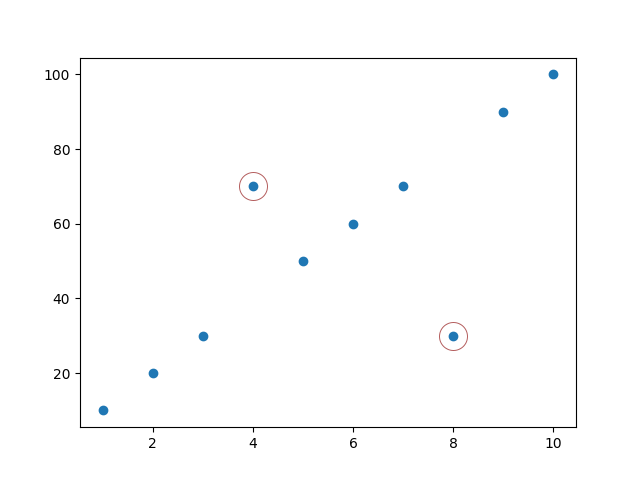
\includegraphics[]{imgs/outliers-example.png}
\caption{An example of outliers in a scatter plot}
\label{fig:prelim:outliers-example}
\end{figure}

In our case we are looking at anomalies in manufacturing. We want to find defects in images of objects and textures.

\section{Image similarity}
\label{sec:prelim:image-similarity}

To allow us to compare inpainted images to original samples from a dataset we want to use objective measures that try to approach a human visual system. For our research we use two measures specifically: Gradient Magnitude Similarity \cite{xue_gradient_2014, zhang_gradient_2017} and Structured Similarity Index \cite{wang_image_2004}.

\subsection{Structured Similarity Index}

This metric uses three features from an image to be able to make a comparison: luminance, contrast and structure. These features are taken from two images $r$ and $d$.

The luminance is an estimation of the mean intensity:

\begin{align}
    \mu_x = \frac{1}{N}\sum_{i=1}^{N}{x_i}
\end{align}

Using $\mu_r$ and $\mu_d$ we can now make a comparison function $l(r, d)$.

\begin{align}
    l(r, d) = \frac{ 2\mu_x\mu_y + C_1 }{ \mu_x^2 + \mu_y^2 + C_1}
\end{align}

$C_1$ is a constant that avoids instability when $\mu_x^2 + \mu_y^2$ is almost zero. In \cite{wang_image_2004} they choose $C_1 = ( K_1 L )^2$ with $L$ being the range of the pixel values and $K_1$ as a small constant.

Next we make an estimation of the contrast for both images:

\begin{align}
    \sigma_r = \left( \frac{1}{N - 1} \sum_{i=1}^{N}{\left( x_i - \mu_r \right)^2} \right)
\end{align}

Using $\sigma_r$ and $\sigma_d$ we can now make a comparison function $c(r, d)$.

\begin{align}
    c(r, d) = \frac{ 2\sigma_r\sigma_d + C_2 }{ \sigma_r^2 + \sigma_d^2 + C_2}
\end{align}

In \cite{wang_image_2004} they choose $C_2 = ( K_2 L )^2$ with $K_2$ as a small constant.

The structure is measured as the covariance divided by the sum of the standard deviation of the images:

\begin{align}
    \sigma_{rd} = \frac{ 1 }{ N - 1 } \sum^N_{i=1}{(r_i - \mu_r)(d_i - \mu_d)} 
\end{align}

\begin{align}
    s(r, d) = \frac{ \sigma_{rd} + C_3 }{ \sigma_r + \sigma_d + C_3}
\end{align}

When we combine these similarity measures of the images the eventual SSIM function looks like this:

\begin{align}
    SSIM(x, y) = \frac{(2\mu_r\mu_d + C_1)(2\sigma_rd + C_2)}{(\mu^2_r + \mu^2_d + C_1)(\sigma^2_r + \sigma^2_d + C_2)}
\end{align}

% https://medium.com/srm-mic/all-about-structural-similarity-index-ssim-theory-code-in-pytorch-6551b455541e

\subsection{Gradient Magnitude Similarity}

The gradient magnitude similarity (GMS) score uses gradient magnitude maps of a ground truth image and a reconstruction. These local quality maps (LQM) are used to calculate a final score by pooling the map using the standard deviation.

The local quality map is computed using the pixel-wise similarity of gradient magnitude maps. These gradient magnitude maps of the original image $r$ and reconstructed image $d$ are obtained by convolving both images with Prewitt filters in the horizontal ($x$) and vertical ($y$) direction. These filters are defined as follows:

\begin{align}
    h_x =
  \left[ {\begin{array}{ccc}
    1/3 & 0 & -1/3\\
    1/3 & 0 & -1/3\\
    1/3 & 0 & -1/3\\
  \end{array} } \right]
  & \, &
    h_y =
  \left[ {\begin{array}{ccc}
    1/3 & 1/3 & 1/3\\
    0 & 0 & 0\\
    -1/3 & -1/3 & -1/3\\
  \end{array} } \right]
\end{align}

The magnitudes at location $i$ for $r$ and $d$ is denoted as $m_r(i)$ and $m_d(i)$:

\begin{align}
    m_r(i) = \sqrt{ (r \ast h_x)^2 (i) + (r \ast h_y)^2 (i) }
\end{align}

\begin{align}
    m_d(i) = \sqrt{ (d \ast h_x)^2 (i) + (d \ast h_y)^2 (i) }
\end{align}

With these gradient magnitude maps we can now compute the GMS:

\begin{align}
    GMS(i) = \frac{2m_r (i) m_d (i) + C}{m^2_r(i) m^2_d(i) + C}
    \label{eq:prelim:gms}
\end{align}

where C is a positive constant for stability, like the values used for the SSIM.